\chapter{Ανάπτυξη εφαρμογών σε GPU}
\label{chapter:gpgpu}
\section{Παράλληλες αρχιτεκτονικές και εφαρμογές}
\noindent Τις τελευταίες δεκαετίες η συντριπτική πλειοψηφία των υπολογιστικών συστημάτων βασίζεται στην φιλοσοφία σχεδιασμού μικροεπεξεργαστών οι οποίοι εμπεριέχουν μία κεντρική μονάδα επεξεργασίας (CPU). Οι επεξεργαστές αυτοί αποφέρουν όλο και αυξανόμενα επίπεδα επιδόσεων τα οποία, τα τελευταία χρόνια, έχουν προσεγγίσει στο επίπεδο του gigaFLOP (του ενός δισεκατομμυρίου εντολών κινητής υποδιαστολής το δευτερόλεπτο) στην οικιακή αγορά και των εκατοντάδων ή χιλιάδων gigaFLOP σε εγκαταστάσεις cluster. Η ταχεία αυτή αύξηση των επιδόσεων έχει επιτρέψει την μεγάλη βελτίωση των δυνατοτήτων του λογισμικού, είτε αυτή μεταφράζεται στην προσθήκη επιπλέον λειτουργιών είτε σε βελτίωση των διεπαφών χρήστη.

Καθώς οι απαιτήσεις απόδοσης του λογισμικού και οι υπολογιστικές ανάγκες των χρηστών αυξάνονται, οι σχεδιαστές επεξεργαστών αντιμετωπίζουν ολοένα αυξανόμενες απαιτήσεις για την ανάπτυξη ταχύτερου επεξεργαστικού υλικού. Οι απαιτήσεις αυτές μέχρι πρόσφατα καλύπτονταν με δύο βασικές και αλληλένδετες σχεδιαστικές επιλογές: Την αύξηση της συχνότητας λειτουργίας των επεξεργαστών και την χρήση ολοένα αυξανόμενων κλιμάκων ολοκλήρωσης. Η μέθοδος αυτή, αν και απέδωσε τα αναμενόμενα για ένα σημαντικό χρονικό διάστημα, αποφέρει σημαντικά μικρότερη αύξηση επιδόσεων τα τελευταία χρόνια (η επιβράδυνση αυτή θεωρείται ότι άρχισε περί το 2003). Προβλήματα υψηλής κατανάλωσης ενέργειας και δυσκολίας απαγωγής της παραγόμενης θερμότητας περιορίζουν σημαντικά τις τεχνικές σχεδιασμού επεξεργαστών. H λύση η οποία έχει υιοθετηθεί από σχεδόν όλους τους κατασκευαστές επεξεργαστών είναι ο σχεδιασμός επεξεργαστών πολλαπλών πυρήνων.

Ένας επεξεργαστής πολλαπλών πυρήνων αποτελείται από δύο ή περισσότερες  πλήρως ανεξάρτητες υπολογιστικές μονάδες, τους πυρήνες, διαμορφωμένες ώστε κάθε μία από αυτές να μπορεί να εκτελέσει πλήρως όλες τις εντολές του συνόλου εντολών του επεξεργαστή. Η σχεδίαση αυτή επιτρέπει στον επεξεργαστή να εκτελεί περισσότερα από ένα νήματα επεξεργασίας. Η παράλληλη επεξεργασία μπορεί να αποφέρει σημαντική αύξηση των υπολογιστικών επιδόσεων σε συγκεκριμένες περιπτώσεις εφαρμογών. Λόγω της σταδιακής μείωσης των περιθωρίων βελτίωσης της απόδοσης ανά πυρήνα, για τους λόγους που προαναφέρθηκαν, η εκμετάλλευση της παραλληλίας είναι το πιο ενεργό πεδίο μελέτης στον σχεδιασμό επεξεργαστών τα τελευταία χρόνια.

Η επίδραση της παραλληλίας στην τεχνολογία λογισμικού είναι εξίσου σημαντική, αν όχι σημαντικότερη, από αυτήν  που ασκεί στον σχεδιασμό του υλικού. Η μεγάλη πλειοψηφία των εφαρμογών που κυκλοφορούν είναι υλοποιημένες με την μορφή ακολουθιακών προγραμμάτων. Ένα ακολουθιακό πρόγραμμα είναι ουσιαστικά μια ακολουθία εντολών οι οποίες πρέπει να εκτελεστούν βήμα-βήμα με συγκεκριμένη σειρά και με το αποτέλεσμα του κάθε βήματος να εξαρτάται άμεσα από τα προηγούμενα. Μία αυστηρά ακολουθιακή ροή εκτέλεσης ενός προγράμματος δεν μπορεί να μοιραστεί ανάμεσα στους πυρήνες ενός πολυπύρηνου επεξεργαστή. Ένα τέτοιο πρόγραμμα δεν μπορεί να επωφεληθεί από την αύξηση επιδόσεων του υλικού που προσφέρει η παραλληλία. Έτσι, η αύξηση της απόδοσης του προγράμματος μπορεί να γίνει μόνο με την βελτίωση της απόδοσης ανά πυρήνα. Η βελτίωση αυτή, όπως προαναφέρθηκε, έχει αργούς ρυθμούς τα τελευταία χρόνια.

H εκμετάλλευση της παραλληλίας του υλικού απαιτεί την ενσωμάτωση νέων πρακτικών στην ανάπτυξη προγραμμάτων. Ένα παράλληλο πρόγραμμα πρέπει να είναι σε θέση να μοιράζει τον φόρτο εργασίας του σε πολλαπλά νήματα επεξεργασίας τα οποία θα συνεργάζονται όπως απαιτείται για την επεξεργασία των δεδομένων του προγράμματος. Τα πολλαπλά αυτά νήματα κατανέμονται από το σύστημα στους πυρήνες του επεξεργαστή (ή επεξεργαστών) και αξιοποιούν την επιτάχυνση που τους παρέχει η παράλληλη δομή του υλικού. Οι τεχνικές ανάπτυξης τέτοιων προγραμμάτων ονομάζονται συνολικά «παράλληλος προγραμματισμός». 

Η ανάπτυξη παράλληλων προγραμμάτων δεν είναι νέο πεδίο έρευνας. Τέτοια προγράμματα αναπτύσσονται από ειδικούς στην υπολογιστική υψηλών επιδόσεων εδώ και πολλές δεκαετίες. Τα προγράμματα αυτά παλαιότερα προορίζονταν για εκτέλεση σε ειδικά σχεδιασμένους υπερυπολογιστές μεγάλης κλίμακας. Μόνο συγκεκριμένες εφαρμογές υψηλής σημασίας μπορούσαν να δικαιολογήσουν την ανάπτυξη τέτοιων συστημάτων. Τα τελευταία χρόνια, με την εξάπλωση των επεξεργαστών πολλαπλών πυρήνων, η ανάπτυξη παράλληλων προγραμμάτων είναι πια γενική ανάγκη. Ο αριθμός των εφαρμογών που απαιτούν παράλληλες υλοποιήσεις έχει αυξηθεί δραματικά. Η αυξανόμενη αυτή ανάγκη έχει χαρακτηριστεί ως «Επανάσταση του ταυτοχρονισμού» (\begin{english}Concurrency Revolution\end{english}). Μια εις βάθος ανάλυση της επίδρασης της αυξανόμενης χρήσης της παραλληλίας στην ανάπτυξη λογισμικού γίνεται στην δημοσίευση ~\cite{Sutter:2005:SCR:1095408.1095421}. 

\section{Οι GPU ως παράλληλοι επεξεργαστές}
\label{chapter:gpucalc}
\noindent Η πιο συνηθισμένη μέθοδος επίτευξης παράλληλης επεξεργασίας στο επίπεδο του υλικού είναι η χρήση πολλαπλών ανεξάρτητων πυρήνων όπως αυτή έχει εφαρμοστεί στις CPU γενικού σκοπού. Η πρώτη γενιά τέτοιων επεξεργαστών περιείχαν δύο πυρήνες, ενώ μέχρι την σύνταξη αυτού του κειμένου είχαν εμφανιστεί υλοποιήσεις με 4,6 και 8 πυρήνες με γενική τάση διπλασιασμού του αριθμού των πυρήνων ανά γενιά επεξεργαστών. Κάθε ένας από αυτούς του πυρήνες είναι πρακτικά ένας ανεξάρτητος επεξεργαστής \textit{πολλαπλής έκδοσης} (multiple issue) με δυνατότητες \textit{εκτέλεσης εκτός σειράς} (\begin{english}out-of-order execution\end{english}) ο οποίος υλοποιεί ολόκληρο το σύνολο εντολών της αρχιτεκτονικής στην οποία βασίζεται. O σχεδιασμός του κάθε πυρήνα διατηρεί τα αρχιτεκτονικά στοιχεία που χρειάζονται για την επιτάχυνση των ακολουθιακών εφαρμογών. Ο κάθε πυρήνας σχεδιάζεται με γνώμονα την μεγιστοποίηση της υπολογιστικής απόδοσης σε ακολουθιακό κώδικα. Η μέθοδος αυτή προορίζεται κυρίως για την μεγιστοποίηση της απόδοσης 
στην περίπτωση της ταυτόχρονης εκτέλεσης πολλαπλών εφαρμογών από τον χρήστη. Στην περίπτωση αυτή οι εφαρμογές κατανέμονται στους διαθέσιμους πυρήνες από το λειτουργικό σύστημα, επιτυγχάνοντας έτσι την εκμετάλλευση της υπολογιστικής ισχύος όλων των πυρήνων και την αύξηση της συνολικής απόδοσης του συστήματος.

Στο δεύτερο μισό της δεκαετίας του 2000 εμφανίστηκε μια εναλλακτική προσέγγιση στην παράλληλη επεξεργασία: η χρήση των GPU στην εκτέλεση υπολογισμών γενικού σκοπού. Η προσέγγιση αυτή βασίζεται στην διαπίστωση ότι η αρχιτεκτονική του υλικού των GPU, η οποία είχε αναπτυχθεί με γνώμονα τις επιδόσεις στους υπολογισμούς γραφικών, μπορούσε να προσαρμοστεί επιτυχώς στην εκτέλεση κάποιων κατηγοριών υπολογισμού γενικού σκοπού επιτυγχάνοντας υψηλές επιδόσεις. Η αρχιτεκτονική αυτή ονομάζεται σχεδιασμός «πολλών πυρήνων» (many-core). Στον σχεδιασμό αυτό βασίζονται πρακτικά όλες οι πρόσφατες GPU από το 2006 και μετά. Ο σχεδιασμός αυτός δίνει μεγαλύτερο βάρος στην μεγιστοποίηση της διεκπεραιωτικής ικανότητας του υλικού στην παράλληλη επεξεργασία. Η αρχιτεκτονική αυτή περιλαμβάνει σημαντικά μεγαλύτερο αριθμό πυρήνων (της τάξης των εκατοντάδων) απλούστερου σχεδιασμού με έμφαση στην επιτάχυνση της παράλληλης επεξεργασίας. 

Παράδειγμα many-core GPU που επιδεικνύει τα βασικά στοιχεία του σχεδιασμού «πολλών πυρήνων» είναι η GT200 της Nvidia η οποία ενσωματώνεται στις κάρτες γραφικών \begin{english}GeForce GTX 280\end{english}. Η GPU αυτή περιέχει 240 «πυρήνες» κάθε ένας από τους οποίους είναι ένας πολυνηματικός επεξεργαστής \textit{μονής έκδοσης} (single issue) με εκτέλεση εντολών σε σειρά (in-order execution). Οι πυρήνες αυτοί ομαδοποιούνται σε ομάδες των 8, εντός των οποίων μοιράζονται μία κοινόχρηστη μονάδα ελέγχου και μία κοινόχρηστη κρυφή (cache) μνήμη εντολών. 

Οι επεξεργαστές που βασίζονται σε αυτό το σχεδιασμό έχουν ξεπεράσει τις «συμβατικές» CPU στην απόδοση εντολών κινητής υποδιαστολής σε πολύ μεγάλο βαθμό από το 2003 και μετά. Με την πάροδο του χρόνου η διαφορά των επιδόσεων αυξάνεται με ταχείς ρυθμούς καθώς η αρχιτεκτονική των GPU εξελίσσεται ταχύτατα και δέχεται μεγάλες βελτιώσεις. Το 2009 η αναλογία διεκπεραιωτικής ικανότητας για πράξεις κινητής υποδιαστολής πλησίαζε το 10 προς 1 μεταξύ GPU και CPU, ενώ οι GPU πλησίαζαν το επίπεδο του ενός teraFLOP. Πρέπει βέβαια να σημειωθεί ότι οι μετρήσεις αυτές δεν μεταφράζονται άμεσα σε επιδόσεις εφικτές σε πραγματικές εφαρμογές. Ωστόσο είναι μια ένδειξη των δυνατοτήτων του υλικού αυτού και της σημασίας που έχει η εκμετάλλευσή τους.

Τα αίτια αυτής της μεγάλης απόκλισης στην απόδοση μεταξύ των δύο σχεδιασμών είναι πολύπλοκα. Ωστόσο, το μεγαλύτερο μέρος της απόκλισης αυτής μπορεί να αποδοθεί σε δύο παράγοντες:
\begin{itemize}
\item Πρώτον, το διαφορετικό βάρος που δίδεται στα επιμέρους τμήματα του επεξεργαστή από τους δύο σχεδιασμούς. Οι CPU έχουν αναπτυχθεί με βάση τις επιδόσεις σε ακολουθιακό κώδικα. Οι σύγχρονοι επεξεργαστές χρησιμοποιούν πολύπλοκες μονάδες ελέγχου πολλαπλών επιπέδων ώστε να επιτραπεί στις εντολές που ανήκουν σε ένα νήμα επεξεργασίας να εκτελεστούν παράλληλα ή σε σειρά διαφορετική από την ονομαστική τους. Επίσης, μεγάλα τμήματα της επιφάνειας του ολοκληρωμένου κυκλώματος μίας σύγχρονης CPU αποτελούνται από κρυφές (cache) μνήμες. Οι μνήμες αυτές προορίζονται για την μείωση της καθυστέρησης πρόσβασης στα δεδομένα της κύριας μνήμης του συστήματος. Τα στοιχεία αυτά είναι σημαντικά για τον ακολουθιακό κώδικα αλλά δεν συνεισφέρουν στην αύξηση της καθαρής ταχύτητας επεξεργασίας. Αντίθετα, οι GPU έχουν αναπτυχθεί με γνώμονα αυτή την ταχύτητα. Ως συνέπεια, χρησιμοποιούν πολύ απλούστερες μονάδες ελέγχου  και αναλογικά ελάχιστες κρυφές μνήμες. Στον σχεδιασμό του ολοκληρωμένου κυκλώματος μίας GPU επικρατούν τα 
επεξεργαστικά στοιχεία. 
\item Δεύτερον, η ταχύτητα της μνήμης. Η κύρια μνήμη (RAM) που χρησιμοποιεί μια CPU χρησιμοποιείται και για την επικοινωνία με τις υπόλοιπες συσκευές του συστήματος. Το γεγονός αυτό, καθώς και κάποιοι περιορισμοί που επιβάλλει η πολυεπίπεδη ιεραρχία μνήμης στην οποία εντάσσεται η μνήμη αυτή, περιορίζουν σημαντικά την μέγιστη ταχύτητα λειτουργίας της. Η μνήμη μίας GPU δεν έχει κανέναν από αυτούς τους περιορισμούς. Κατά συνέπεια είναι εφικτή η λειτουργία της σε πολύ μεγαλύτερες ταχύτητες. Ενδεικτικά μπορούμε να αναφέρθεί ότι τα τελευταία χρόνια η μέγιστη διεκπεραιωτική ικανότητα της κύριας μνήμης για CPU (πρότυπο DDR3) έχει παραμείνει σταθερή κοντά στα 50 GB/s, ενώ οι μνήμες της τελευταίας γενιάς GPU (πρότυπο GDDR5) έχουν πλησιάσει τα 150 GB/s.
\end{itemize}
Η σχεδιαστική φιλοσοφία των GPU διαμορφώθηκε από τις απαιτήσεις της εξαιρετικά ανταγωνιστικής αγοράς των τριδιάστατων γραφικών. Η αγορά αυτή ασκεί μεγάλες πιέσεις στους σχεδιαστές του υλικού για την μεγιστοποίηση της απόδοσης στις πράξεις κινητής υποδιαστολής, όπως προαναφέρθηκε. Για να είναι εφικτή η μεγιστοποίηση αυτή οι σχεδιαστές  έχουν στραφεί στην λύση του εξαιρετικά μεγάλου αριθμού νημάτων παράλληλης επεξεργασίας. Το υλικό εκμεταλλεύεται τον μεγάλο αριθμό νημάτων ώστε να υπάρχει μεγάλο ποσοστό αξιοποίησης των υπολογιστικών του στοιχείων σε κάθε κύκλο επεξεργασίας. Αυτό γίνεται επειδή όταν κάποια από τα νήματα βρίσκονται σε αναμονή για μεταφορά στοιχείων από και προς την μνήμη, τα υπολογιστικά στοιχεία μπορούν να απασχοληθούν με τους υπολογισμούς των υπολοίπων νημάτων. Με τον τρόπο αυτό επιτυγχάνεται η απόκρυψη των καθυστερήσεων (\begin{english}latency hiding\end{english}) οι οποίες δημιουργούνται από τις προσβάσεις στη μνήμη. Η σχεδιαστική αυτή επιλογή έχει ιδιαίτερη σημασία για τις επιδόσεις των 
προγραμμάτων σε GPU λόγω της απλούστερης ιεραρχίας μνήμης και της ύπαρξης λιγότερης κρυφής μνήμης σε σχέση με τις CPU. Συνολικά, ο σχεδιασμός αυτός έχει οδηγήσει στην δημιουργία του όρου «μαζικά παράλληλος επεξεργαστής» (\begin{english}massively parallel processor\end{english}) ως χαρακτηρισμό για τις GPU.

\begin{figure}[b!]
\centering{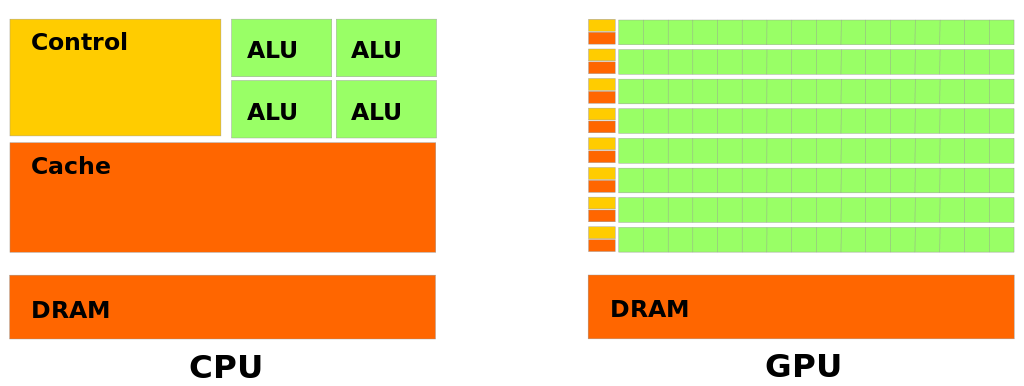
\includegraphics[scale=0.4]{./graphics/cpugpucomparison.png}}
\captionsetup{singlelinecheck=off}
\caption[Σύγκριση αρχιτεκτονικών στοιχείων CPU και GPU.]{Σύγκριση αρχιτεκτονικών στοιχείων CPU και GPU. Με κίτρινο χρώμα εμφανίζονται οι μονάδες ελέγχου,με πορτοκαλί τα στοιχεία μνήμης και με πράσινο τα υπολογιστικά στοιχεία. Διακρίνεται η μεγαλύτερη έμφαση που δίδεται στα υπολογιστικά στοιχεία (ALU) στις GPU σε αντίθεση με την μεγαλύτερη έκταση των μνημών και μονάδων ελέγχου στις CPU.}
\label{fig6}
\end{figure}
Η μορφή της παράλληλης επεξεργασίας που εφαρμόζεται στις GPU ανήκει στην κατηγορία \begin{english}SIMD (Single Instruction Multiple Data)\end{english}. Συνοπτικά, σε αυτή την εκδοχή της παραλληλίας κάθε εντολή εκτελείται παράλληλα σε ένα μεγάλο εύρος δεδομένων. Οι επεξεργαστές SIMD συνδυάζουν την κάθε μονάδα ελέγχου που περιέχουν με έναν αριθμό μονάδων υπολογισμού. Κάθε εντολή που αποκωδικοποιείται από την μονάδα ελέγχου εκτελείται παράλληλα από καθεμία  από τις συνδυασμένες μονάδες σε διαφορετικό τμήμα δεδομένων. Παράδειγμα υπολογισμού που μπορεί να παραλληλοποιηθεί εύκολα σε έναν επεξεργαστή SIMD είναι η πρόσθεση δύο πινάκων. Η τιμή κάθε στοιχείου του τελικού πίνακα εξαρτάται μόνο από την τιμή των αντίστοιχων κελιών στους αρχικούς πίνακες. Ένας επεξεργαστής ακολουθιακής αρχιτεκτονικής θα έπρεπε να διατρέξει όλα τα κελιά και να εφαρμόσει την πράξη της πρόσθεσης σε κάθε ένα για να υπολογίσει τον τελικό πίνακα. Αντίθετα, σε έναν επεξεργαστή SIMD μία εντολή πρόσθεσης μπορεί να εφαρμοστεί σε ολόκληρο τον πίνακα.
 Κάθε υπολογιστικό στοιχείο υπολογίζει παράλληλα με τα υπόλοιπα την τιμή του στοιχείου που του αντιστοιχεί.  

Η απόδοση δεν είναι ο μόνος λόγος για το αυξημένο ενδιαφέρον για την χρήση των GPU ως παράλληλων επεξεργαστών. Άλλοι παράγοντες έχουν την ίδια ή και μεγαλύτερη σημασία. Ο κυριότερος από αυτούς είναι το γεγονός ότι οι GPU έχουν ήδη μεγάλη παρουσία στην αγορά της πληροφορικής. Ο αριθμός των επεξεργαστών κάποιου τύπου οι οποίοι χρησιμοποιούνται ήδη στην αγορά ονομάζεται «εγκατεστημένη βάση» ενός επεξεργαστή. Η εγκατεστημένη βάση ενός είδους επεξεργαστή έχει μεγάλη σημασία στις αποφάσεις της αγοράς σχετικά με την αξιοποίησή του. Αυτό ισχύει επειδή το κόστος της ανάπτυξης λογισμικού για κάποιον επεξεργαστή δικαιολογείται από το πλήθος των πελατών στο οποίο απευθύνεται. Οι εφαρμογές που προορίζονται για κάποιον επεξεργαστή με μικρή εγκατεστημένη βάση απευθύνονται σε μικρότερο κοινό και έχουν μικρότερη πιθανότητα να επιτύχουν εμπορικά. Αυτό αποτελούσε ένα σημαντικό πρόβλημα για τις παλαιότερες μορφές παράλληλων συστημάτων τα οποία βασίζονταν σε «εξωτικές» αρχιτεκτονικές με μικρή απήχηση στην αγορά. Μόνο ένα μικρό 
ποσοστό ειδικών εφαρμογών ήταν οικονομικά βιώσιμο σε αυτά τα συστήματα. Οι GPU ανατρέπουν πλήρως αυτή την τάση. Λόγω της δημοφιλίας τους στην αγορά των προσωπικών υπολογιστών οι GPU κατέχουν ήδη μια γιγάντια εγκατεστημένη βάση. Εκατοντάδες εκατομμύρια GPU υπάρχουν ήδη σε  υπολογιστές σε όλο τον κόσμο, καθιστώντας την μαζικά παράλληλη επεξεργασία διαθέσιμη στο κοινό και οικονομικά ελκυστική για τους σχεδιαστές λογισμικού.

Άλλος παράγοντας που στρέφει το ενδιαφέρον της αγοράς προς τις GPU είναι η ευκολία προσαρμογής τους σε μεγάλο εύρος περιβαλλόντων. Η πλειοψηφία του παράλληλου λογισμικού πριν το 2006 προοριζόταν προς εκτέλεση σε  εγκαταστάσεις server μεγάλης κλίμακας ή σε cluster πολλαπλών μηχανημάτων. Αυτό περιόριζε την χρήση τους σε περιβάλλοντα με περιορισμούς χώρου ή υποδομών. Ένα χαρακτηριστικό παράδειγμα των προβλημάτων που επέβαλλε ο περιορισμός αυτός είναι η χρήση παράλληλων επεξεργαστών στην επεξεργασία δεδομένων που προέρχονται από μαγνητική τομογραφία. Η μαγνητική τομογραφία έχει μεγάλες υπολογιστικές απαιτήσεις για την παραγωγή αξιόπιστων απεικονίσεων υψηλής ανάλυσης. Αν και τα κλασικά παράλληλα υπολογιστικά συστήματα ήταν ικανά να καλύψουν αυτές τις απαιτήσεις, το μέγεθός τους καθιστούσε αδύνατη την χρήση τους σε ιατρικά περιβάλλοντα. Αντίθετα, ένα σύστημα βασισμένο σε GPU εγκατεστημένες σε ένα πλαίσιο απλού οικιακού υπολογιστή μπορεί να παρέχει συγκρίσιμη ή και μεγαλύτερη ισχύ χωρίς τους περιορισμούς των 
μεγάλων εγκαταστάσεων. Τέτοια συστήματα έχουν ήδη εμφανιστεί στην αγορά από διάφορους κατασκευαστές.      

Τέλος, ένας ακόμα παράγοντας που έχει δημιουργήσει ενδιαφέρον για την μεταφορά κάποιων αριθμητικών εφαρμογών σε GPU είναι η υποστήριξη από τις νέες GPU του προτύπου του Ινστιτούτου Ηλεκτρολόγων και Ηλεκτρονικών Μηχανικών (\begin{english}Institute of Electrical and Electronics Engineers, IEEE)\end{english} σχετικά με τους υπολογισμούς κινητής υποδιαστολής. Το πρότυπο αυτό (ΙΕΕΕ 754) εξασφαλίζει ότι τα αποτελέσματα των υπολογιστών θα είναι προβλέψιμα και πανομοιότυπα μεταξύ επεξεργαστών από διαφορετικούς κατασκευαστές. Αν και οι παλιότερες γενιές GPU  δεν είχαν εγγυημένη υποστήριξη σε αυτό το πρότυπο, σχεδόν όλες όσες σχεδιάστηκαν μετά το 2006 το εφαρμόζουν πλήρως. Παρομοίως, αν και οι παλαιότερες γενιές GPU υποστήριζαν μόνο αριθμούς κινητής υποδιαστολής μονής ακρίβειας, όσες από αυτές σχεδιάστηκαν μετά το 2008 υποστηρίζουν πλήρως και αριθμούς διπλής ακρίβειας. Η αλλαγή αυτή τις καθιστά πολύ πιο χρήσιμες σε επιστημονικές εφαρμογές όπου η μεγαλύτερη ακρίβεια είναι σημαντικότατη.   

Οι παράγοντες που αναφέρθηκαν έχουν δημιουργήσει σημαντικό ενδιαφέρον σε πολλούς σχεδιαστές εφαρμογών για την μεταφορά κάποιων υπολογιστικά εντατικών τμημάτων των εφαρμογών τους σε GPU. Γενικά, τα τμήματα του λογισμικού που απαιτούν την μεγαλύτερη ποσότητα υπολογιστικής ισχύος είναι και αυτά που επιδέχονται την μεγαλύτερη παραλληλοποίηση. Αυτό ισχύει επειδή ένα μεγαλύτερο φορτίο υπολογισμών μπορεί να διαιρεθεί πιο εύκολα σε διαφορετικά νήματα επεξεργασίας σε σχέση με κάποιο μικρότερο. Ως αποτέλεσμα όλων αυτών ένα συνεχώς αυξανόμενο ποσοστό εφαρμογών σχεδιάζεται σε δύο τμήματα: ακολουθιακό κώδικα που προορίζεται προς εκτέλεση σε CPU για τα μη παραλληλοποιήσιμα τμήματα του υπολογισμού, και παράλληλο κώδικα για GPU που αναλαμβάνει τα υπολογιστικά «βαριά» τμήματα. Η εφαρμογή που αναπτύχθηκε στα πλαίσια αυτής της εργασίας ανήκει σε αυτή την κατηγορία.

Μέχρι το 2006, η ανάπτυξη λογισμικού προορισμένου για να λειτουργεί μέσω της συνεργασίας GPU και CPU παρουσίαζε σημαντικές δυσκολίες. Ο μόνος τρόπος προγραμματισμού των GPU που ήταν διαθέσιμος ήταν η χρήση των διεπαφών προγραμματισμού εφαρμογών\begin{english} (application programming interfaces, APIs)\end{english} που προορίζονταν για την παραγωγή γραφικών, όπως τα Direct3D και OpenGL. Οι διεπαφές αυτές δεν είχαν σχεδιαστεί για προγραμματισμό γενικού σκοπού και, κατά συνέπεια, περιόριζαν σημαντικά τις δυνατότητες των εφαρμογών τους και παρείχαν ένα δύστροπο προγραμματιστικό περιβάλλον. Παρ' όλα αυτά, οι προγραμματιστικές προσπάθειες που έγιναν σε αυτά τα περιβάλλοντα και οι παράγοντες που προαναφέραμε έκαναν ορατή στις εταιρίες παραγωγής GPU την ανάγκη του ανοίγματος του υλικού τους στον προγραμματισμό γενικού σκοπού. Το άνοιγμα αυτό, που απαίτησε σημαντικές αλλαγές στο υλικό και το λογισμικό των GPU, έγινε με την δημιουργία των πρώτων ολοκληρωμένων περιβαλλόντων ανάπτυξης εφαρμογών σε GPU.
   
\section{Περιβάλλοντα ανάπτυξης εφαρμογών σε GPU}
\label{chapter:apis}
\noindent Τις δεκαετίες του '80 και '90 η μορφή των GPU ήταν σημαντικά διαφορετική από την σημερινή. Οι GPU της εποχής αυτής μπορούσαν να εκτελέσουν μόνο μια συγκεκριμένη σειρά τυποποιημένων μετασχηματισμών στα δεδομένα γραφικών που δέχονταν. Αν και η λειτουργία τους επιδεχόταν κάποιο επίπεδο προσαρμογής από την εκάστοτε εφαρμογή, αυτή περιοριζόταν από το περιορισμένο εύρος λειτουργιών που εκτελούσαν. Ουσιαστικά αυτό σήμαινε ότι δεν υπήρχε μέθοδος προγραμματισμού των GPU για πεδία πέρα από τα γραφικά. Την εποχή αυτή αναπτύχθηκαν και οι κοινές διεπαφές προγραμματισμού οι οποίες επικρατούν ακόμα στο πεδίο των τριδιάστατων γραφικών: Η Direct3D, τμήμα του γενικότερου πακέτου πολυμέσων DirectX της εταιρίας Microsoft, και η OpenGL, μία ανοικτή διεπαφή προγραμματισμού γραφικών που αναπτύχθηκε συλλογικά από  διάφορους κατασκευαστές και επιβλέπεται από την Khronos Group, μια κοινοπραξία στην οποία συμμετέχουν διάφορες εταιρίες του κλάδου της πληροφορικής.

Σταδιακά, με τη εξέλιξη των αρχιτεκτονικών των GPU και της αύξηση των απαιτήσεων της αγοράς γραφικών, διαμορφώθηκε η ανάγκη του ανοίγματος του άμεσου προγραμματισμού των εσωτερικών λειτουργιών των GPU στους προγραμματιστές εφαρμογών γραφικών. Η αλλαγή αυτή έγινε με κύριο σκοπό την παραγωγή καλύτερης ποιότητας τριδιάστατων γραφικών. Η τάση αυτή άρχισε με την γενιά των καρτών γραφικών Geforce 3 της εταιρίας Nvidia το 2003 η οποία παρείχε πρόσβαση σε ένα από τα στάδια των γραφικών μετασχηματισμών. Το υπόλοιπο της αγοράς  ακολούθησε παρόμοιες τακτικές. Τα επόμενα χρόνια σταδιακά το σύνολο των λειτουργιών των GPU έγινε άμεσα προγραμματίσιμο, ενώ ανάλογη πρόοδος σημειώθηκε και στα API για την εκμετάλλευση των νέων αυτών δυνατοτήτων του υλικού.

Τα χρόνια αυτά η δυνατότητα εκμετάλλευσης των νέων GPU για την εκτέλεση  αριθμητικών εφαρμογών μεγάλης κλίμακας είχε ήδη γίνει εμφανής σε διάφορους ερευνητές, κυρίως στο πλαίσιο επιστημονικών εφαρμογών. Η μεθοδολογία που χρησιμοποιούσαν βασιζόταν στην χρήση των API γραφικών. Η κύρια ιδέα της μεθόδου αυτής ήταν η χρήση των δομών επεξεργασίας γραφικών της GPU με την μετατροπή των εφαρμογών στην μορφή γραφικών υπολογισμών. Οι επιθυμητοί υπολογισμοί μετασχηματίζονταν σε ισοδύναμες εντολές επεξεργασίας γραφικών στοιχείων. Έτσι ήταν δυνατή η χρήση των GPU για επεξεργασία γενικού σκοπού χρησιμοποιώντας την υπάρχουσα υποδομή επεξεργασίας γραφικών. Γι' αυτό η μεθοδολογία αυτή ονομάστηκε GPGPU (συντομογραφία του \begin{english}General Purpose computing on GPUs\end{english}, υπολογισμός γενικού σκοπού σε GPU).

Οι περιορισμοί της μεθοδολογίας GPGPU δεν άργησαν να γίνουν εμφανείς. Ούτε το υλικό ούτε τα API της εποχής ήταν προσαρμοσμένα στην επεξεργασία αυτού του είδους. Το προγραμματιστικό περιβάλλον επέβαλλε μεγάλους περιορισμούς στον τρόπο χρήσης της μνήμης της GPU. Επιπλέον, η είσοδος και έξοδος δεδομένων μπορούσε να πραγματοποιηθεί μόνο με τους αυστηρά ορισμένους τρόπους τους οποίους οι GPU χρησιμοποιούν για την μεταφορά δεδομένων γραφικών. Όλα αυτά συντελούσαν στην διαμόρφωση ενός δύστροπου προγραμματιστικού περιβάλλοντος. Η χρήση της μεθοδολογίας GPGPU τελικά περιορίστηκε σε λίγες επιστημονικές εφαρμογές.

Η μεγάλη στροφή προς τον υπολογισμό σε GPU πραγματοποιήθηκε τα έτη 2006-2007. Τον Νοέμβριο του 2006 η εταιρία ATI παρουσίασε το πρώτο API που απευθυνόταν αποκλειστικά στον υπολογισμό με GPU με την ονομασία Close To Metal (\url{http://en.wikipedia.org/wiki/Close_to_Metal}). Το API αυτό παρείχε άμεση πρόσβαση στις χαμηλού επιπέδου λειτουργίες της GPU με τεχνικές ανάλογες του προγραμματισμού CPU, διευκολύνοντας σημαντικά την ανάπτυξη εφαρμογών. Το επόμενο βήμα ήρθε με την κυκλοφορία των GPU βασισμένων στην αρχιτεκτονική Tesla από την Νvidia το 2007. Η αρχιτεκτονική αυτή αποτελεί το πρώτο παράδειγμα GPU σχεδιασμένης με την λογική του «μαζικά παράλληλου επεξεργαστή». Στις κλασικές αρχιτεκτονικές GPU τα στάδια επεξεργασίας των γραφικών αντιστοιχούσαν σε διαφορετικά τμήματα του υλικού. Καθένα από αυτά τα τμήματα ήταν εξειδικευμένο σε μόνο μία λειτουργία η οποία ήταν και η μοναδική που μπορούσε να εκτελέσει. Η καινοτομία της Tesla ήταν η δόμηση της GPU ως μίας σειράς ανεξάρτητων, πλήρως προγραμματίσιμων παράλληλων 
επεξεργαστών πολλαπλών λειτουργιών. Σε κάθε έναν από αυτούς μπορεί να  ανατεθεί δυναμικά να εκτελέσει οποιοδήποτε πιθανή επεξεργασία που καλύπτεται από την αρχιτεκτονική της, γραφική ή όχι. Μαζί με τα πρώτα προϊόντα βασισμένα στην Tesla κυκλοφόρησε και το πρώτο ολοκληρωμένο περιβάλλον προγραμματισμού σε GPU, το CUDA (\url{http://www.nvidia.com/object/cuda_home_new.html}) της Nvidia. Το CUDA επιτρέπει την εύκολη ανάπτυξη εφαρμογών για τις GPU της Nvidia χρησιμοποιώντας μια γλώσσα βασισμένη άμεσα στη C (με στοιχεία C++ στις νεότερες εκδόσεις).

Η πρώτη εναλλακτική λύση στο CUDA εμφανίστηκε το Νοέμβριο του 2008 και ονομάζεται OpenCL (\url{http://www.khronos.org/opencl/}). Το OpenCL είναι ένα ανοιχτό πρότυπο «ετερογενούς προγραμματισμού». Με την όρο αυτό χαρακτηρίζεται η μέθοδος προγραμματισμού η οποία επιτρέπει την δημιουργία κώδικα που μπορεί να εκτελείται σε εντελώς διαφορετικές αρχιτεκτονικές επεξεργαστών (CPU, GPU, FPGA). O κύριος σχεδιαστικός στόχος του OpenCL είναι η εκμετάλλευση των ιδιαίτερων χαρακτηριστικών της κάθε αρχιτεκτονικής για την επίτευξη της μέγιστης δυνατής απόδοσης. Το OpenCL αναπτύχθηκε αρχικά από την εταιρία Apple και στην συνέχεια διαμορφώθηκε σε πρότυπο από μια ομάδα εταιριών που περιλαμβάνει τις AMD, IBM, Intel και Nvidia. Το πρότυπο OpenCL σήμερα επιβλέπεται και εξελίσσεται από την κοινοπραξία Khronos Group. Η γλώσσα προγραμματισμού του OpenCL βασίζεται στην C και ιδιαίτερα στο πρότυπο C99. Υλοποιήσεις του OpenCL υπάρχουν για ένα μεγάλο εύρος υλικού από διάφορους κατασκευαστές.

Η τριάδα των σύγχρονων API ολοκληρώνεται με το \begin{english}DirectCompute\end{english}. Το \begin{english}DirectCompute\end{english} είναι δημιούργημα της Microsoft και πρωτοεμφανίστηκε το 2009, παράλληλα με την κυκλοφορία της έκδοσης 11 του DirectX. Αποτελεί επέκταση του Direct3D, ενός ήδη υπάρχοντος API για την δημιουργία τριδιάστατων γραφικών, προσθέτοντας σε αυτό δυνατότητες υπολογισμού γενικού σκοπού.

Στην ανάπτυξη της εργασίας αυτής έχει χρησιμοποιηθεί το πρότυπο \begin{english}OpenCL\end{english}. Η απόφαση αυτή στηρίχθηκε κυρίως στην ευρεία συμβατότητα του \begin{english}OpenCL\end{english} με συσκευές διαφορετικών κατασκευαστών. 

Το περιεχόμενο των ενοτήτων \ref{chapter:gpucalc} και \ref{chapter:apis} βασίζεται στα στοιχεία του βιβλίου ~\cite{MassivelyParallel}, κεφάλαια 1 και 2.


\section{Το πρόβλημα τομής ευθείας-τετραέδρου σε GPU}
\label{chapter:openclraytetra}
\noindent Όπως αναφέρθηκε στο Κεφάλαιο 1, η ύπαρξη λύσεων υψηλών επιδόσεων για το πρόβλημα τομής ευθείας-τετραέδρου είναι σημαντικότατη για ένα μεγάλο εύρος εφαρμογών. Καθώς οι αλγόριθμοι που παρουσιάστηκαν στο κεφάλαιο \ref{chapter:algs} βασίζονται σχεδόν εξ' ολοκλήρου σε υπολογισμούς κινητής υποδιαστολής, οι επιδόσεις των GPU σε αυτό τον τομέα δικαιολογούν άμεσα την σκοπιμότητα της δημιουργίας μίας υλοποίησης των αλγορίθμων προσαρμοσμένης στην επεξεργασία με GPU.

Το πρώτο βήμα για την δημιουργία της υλοποίησης αυτής είναι η έκφραση του προβλήματος σε κάποια μορφή προσαρμοσμένη στην παράλληλη επεξεργασία. Ένας τρόπος να επιτευχθεί αυτό θα ήταν η παραλληλοποίηση των τριών μορφών των αλγορίθμων που παρουσιάστηκαν στην ενότητα \ref{chapter:algs_general}, δηλαδή η μετατροπή τους με τέτοιο τρόπο ώστε τα επιμέρους τμήματα τους να μπορούν να εκτελεστούν ταυτόχρονα σε διαφορετικά υπολογιστικά στοιχεία της GPU. Η μορφή 0 των αλγορίθμων μπορεί να προσαρμοστεί εύκολα σε μια τέτοια μέθοδο. Στην μορφή αυτή, ο έλεγχος τομής κάθε επιμέρους έδρας του τετραέδρου με την ευθεία είναι ανεξάρτητος από τα αποτελέσματα των ελέγχων των υπολοίπων εδρών. Ως αποτέλεσμα, οι έλεγχοι αυτοί μπορούν να εκτελεστούν παράλληλα. Στον αλγόριθμο, όπως αυτός εμφανίζεται στην ενότητα \ref{chapter:raytetraint}, αυτό αντιστοιχεί σε παράλληλη εκτέλεση του περιεχομένου του βρόχου for για τις διάφορες τιμές του i, μεταφέροντας την διάκριση μεταξύ $F_{enter}$ και $F_{leave}$ εκτός του βρόχου αυτού. Οι 
βελτιστοποιημένες  μορφές 1 και 2, αντίθετα, δεν μπορούν να προσαρμοστούν εύκολα στην παράλληλη επεξεργασία. Στις μορφές αυτές υπάρχει άμεση εξάρτηση του τρόπου ελέγχου της κάθε έδρας από τα δεδομένα που παράγονται κατά των έλεγχο των υπολοίπων, κάνοντας αδύνατη την παράλληλη εκτέλεση των διάφορων ελέγχων έδρας. Επίσης, η σύνθετη ροή ελέγχου σε αυτές τις μορφές καθιστά δύσκολη και την παραλληλοποίηση των επιμέρους εσωτερικών τμημάτων του ελέγχου έδρας. Για αυτούς τους λόγους η μέθοδος αυτή απορρίφθηκε.  

Η προσέγγιση που επιλέχθηκε για την παραλληλοποίηση του προβλήματος είναι ταυτόχρονη εκτέλεση του εκάστοτε αλγορίθμου για έναν μεγάλο αριθμό ζευγών ευθείας-τετραέδρου. Κάθε νήμα επεξεργασίας που δημιουργείται στην GPU αναλαμβάνει ολόκληρη την διερεύνηση της τομής ενός ζεύγους. Πρακτικά αυτό σημαίνει ότι σε κάθε κύκλο ρολογιού στην GPU βρίσκονται υπό εκτέλεση δεκάδες ή εκατοντάδες χιλιάδες στιγμιότυπα των αλγορίθμων. Η προσέγγιση αυτή προτιμήθηκε επειδή:
\begin{itemize}
\item Προσαρμόζεται εύκολα στις προγραμματιστικές μεθόδους που χρησιμοποιούνται από τα περιβάλλοντα ανάπτυξης εφαρμογών σε GPU. Όλα τα σύγχρονα περιβάλλοντα ανάπτυξης βασίζονται σε μια νοοτροπία χρήσης της GPU η οποία απορρέει από την παραλληλία SIMD. Σε αυτή, ένα υπολογιστικά σύνθετο κομμάτι κώδικα το οποίο ονομάζεται πυρήνας (kernel) εκτελείται από κάθε νήμα επεξεργασίας της GPU. Κάθε στιγμιότυπο του πυρήνα λαμβάνει διαφορετικά δεδομένα εισόδου από την κύρια μνήμη του συστήματος με βάση τον αριθμό του. Παρομοίως, τα δεδομένα εξόδου κάθε πυρήνα γράφονται πίσω στην κύρια μνήμη σε διαφορετικές θέσεις. Δημιουργώντας ένα πυρήνα ο οποίος περιλαμβάνει ολόκληρο τον έλεγχο τομής και αποθηκεύοντας τα στοιχεία των ζευγών ευθειών και τετράεδρων με κατάλληλο τρόπο στη μνήμη μπορεί να κατασκευαστεί μια παράλληλη υλοποίηση χωρίς μεγάλης κλίμακας αλλαγές στους αλγορίθμους. 
\item Ταιριάζει με τις κοινές περιπτώσεις χρήσης των αλγορίθμων. Σε όλα τα τυπικά σενάρια εφαρμογών στα οποία χρειάζεται η εύρεση τομής ευθείας-τετραέδρου χρησιμοποιείται μεγάλος αριθμός ζευγών, για παράδειγμα κατά την εκπομπή ακτίνων (ray casting) ενός μοντέλου αποτελούμενου από τετράεδρα. Στις εφαρμογές αυτές έχει μεγάλη σημασία η διεκπεραιωτική ικανότητα του συστήματος, δηλαδή ο αριθμός ζευγών που εξετάζεται ανά μονάδα χρόνου. Ο σχεδιασμός που επιλέχθηκε βελτιστοποιεί το παραγόμενο πρόγραμμα προς αυτή την κατεύθυνση.
\item Δημιουργεί ένα «βαρύ» επεξεργαστικό φορτίο το οποίο μπορεί να κατανεμηθεί καλύτερα στα επεξεργαστικά στοιχεία της GPU και να   εκμεταλλευτεί τις δυνατότητες τους.

\end{itemize}


         